\documentclass[border=10pt]{standalone}
\usepackage{tikz}

\begin{document}
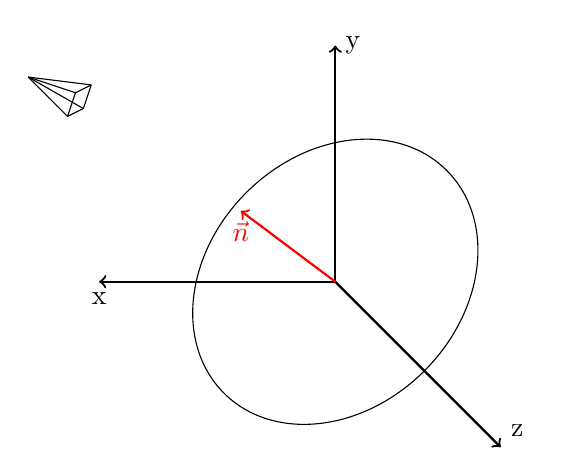
\begin{tikzpicture}
 
  \coordinate (O) at (0,0);
  \coordinate (X) at (-3,0);
  \coordinate (Y) at (0,3);
  \coordinate (Z) at (2.1,-2.1);
  
  \draw [->][thick] (O) -- (X) node [below] {x};
  \draw [->][thick] (O) -- (Y) node [right] {y};
  \draw [->][thick] (O) -- (Z) node [above right] {z};
  
  
  \coordinate (n) at (-1.2, 0.9);
  \draw [->][thick, red] (O) -- (n) node [below] {$\vec{n}$};
  
  \draw (O) ellipse [x radius=1.6, y radius=2, rotate=-45];
  
  
  % camera
  \coordinate (CO) at (-3.9, 2.6);
  \coordinate (CA) at (-3.3, 2.4);
  \coordinate (CB) at (-3.4, 2.1);
  \coordinate (CC) at (-3.2, 2.2);
  \coordinate (CD) at (-3.1, 2.5);
  
  \draw (CO) -- (CA);
  \draw (CO) -- (CB);
  \draw (CO) -- (CC);
  \draw (CO) -- (CD);
  
  \draw (CA) -- (CB);
  \draw (CB) -- (CC);
  \draw (CC) -- (CD);
  \draw (CD) -- (CA);
  
 
\end{tikzpicture}
\end{document}
